%\documentclass[prb,showpacs,showkeys,preprint]{revtex4}
\documentclass[prb,showpacs,showkeys,twocolumn]{revtex4}

	\usepackage[ansinew]{inputenc}
	\usepackage{ae}
	
	\usepackage{SIunits}
	\usepackage{graphicx}
	\graphicspath{{./figuras/}}
		
	%-------------------------------------------------------------------------
	% Acostume-se a utilizar o pacote amsmath. Ele define um sem-número de
	% comandos específicos para o modo matemático, entre outros. As melhores
	% expressões matemática você construirá com este pacote!
	%-------------------------------------------------------------------------
	\usepackage{amsmath}

	%-------------------------------------------------------------------------
	% O pacote natbib reimplementa o comando \cite e define vários outros
	% similares, visando produzir os mais diversos formatos de citações.
	%-------------------------------------------------------------------------
	\usepackage{natbib}
	
	%-------------------------------------------------------------------------
	% Os comandos \ttau e \tauphi abaixo eu defini não só para poupar digitação,
	% mas também para garantir homogeneidade nos símbolos utilizados. Isto é,
	% basta utilizar \ttau e \tauphi que terei certeza de que eles serão todos
	% iguais... eu não corro o risco de errar a digitação e obter símbolos 
	% diferentes para entes físicos iguais.
	%-------------------------------------------------------------------------
	\newcommand{\ttau}   {\ensuremath{\tau_t}}
	\newcommand{\tauphi} {\ensuremath{\tau_\varphi}}

\begin{document}

	\title{Anomalous dephasing scattering rate of two-dimensional electrons
	in double quantum-well structures}
	
	\author{I. R. Pagnossin}
	\email{irpagnossin@usp.br}
	\affiliation{Instituto de Física da Universidade de São Paulo,
	Laboratório de Novos Materiais Semicondutores (LNMS)\\CP 66318, 05315-970,
	São Paulo, SP, Brazil}
	
	\author{A. K. Meikap}
	\email{meikapnitd@yahoo.com}
	\affiliation{Department of Physics, National Institute of Technology,
	Durgapur-713209, W.B., India}
	
	\author{T. E. Lamas}
	\author{G. M. Gusev}
	\affiliation{Instituto de Física da Universidade de São Paulo,
	Laboratório de Novos Materiais Semicondutores (LNMS)\\CP 66318, 05315-970,
	São Paulo, SP, Brazil}
		
	\author{J.-C. Portal}
	\affiliation{GHMFL-CNRS, BP-166, F-38042, Grenoble, Cedex 9, INSA-Toulouse,
	31077, Cedex 4, and Institute Universitaire de France, Toulouse, France}
	
	\date{\today}

%----------------------------------
% ABSTRACT
%----------------------------------
\begin{abstract}

	The results on the measurement of electrical conductivity and	magnetoconductivity of a GaAs double quantum-well between $0.5$ and \unit{1.1}{\kelvin} are reported. The zero magnetic field conductivity is	well described from	the point of view of contributions made by both the weak-localization and	electron-electron interaction. At low field and low temperature, the magnetoconductivity is dominated by the weak localization effect only. Using the weak localization method, we have determined the electron dephasing times $\tauphi$ and tunneling times $\ttau$. Concerning tunneling, we concluded that $\tau_t$ presents a minimum around the balance point, as expected; concerning dephasing, we observed an anomalous dependence on temperature and conductivity (or elastic mean free path) of $\tauphi$. This anomalous behavior cannot be explained in terms of the prevailing concepts for the electron-electron interaction in the high-mobility two-dimensional electron systems.
	
\end{abstract}

\pacs{73.63.Hs, 73.63.Kv, 72.15.R, 71.70.Ej, 71.10.Ay}

\keywords{
	Quantum-well,
	Weak-localization,
	Dephasing scattering rate,
	Fermi-liquid model}
	
\maketitle

%----------------------------------
% INTRODUCTION
%----------------------------------
\section{INTRODUCTION}

	In the course of the last two decades, it has been established that the constructive interference of phase coherent electronic waves propagating along a closed path in opposite directions leads to a weak localization (WL) of the conduction electrons. The main experimental signature of this effect is a positive magnetoconductance at low magnetic field due to the breaking of time reversal symmetry induced by a magnetic field applied perpendicular to the plane of the two-dimensional electron gases (2DEG).

	In addition, theoretical modeling allows one to estimate the dephasing time ($\tauphi$) from the experimental magnetoconductivity of weakly disordered conductors\rlap{.}\cite{Abrahams:1979,Anderson:1980,Hikami:1980} Furthermore, this work has been extended to high mobility 2DEG systems during the last decade to determine the dephasing scattering time. The electron dephasing time is one of the most important characteristics of semiconductor samples because it sets the rate at which the quantum mechanical properties of the microscopic system shifts to the classical behavior and also provides information for the microscopic electron-electron and electron-phonon interactions.

%----------------------------------
% EXPERIMENTAL TECHNIQUES
%----------------------------------
\section{EXPERIMENTAL TECHNIQUES}

	Blá blá blá...
	
	\begin{figure}
		\centering
		\fbox{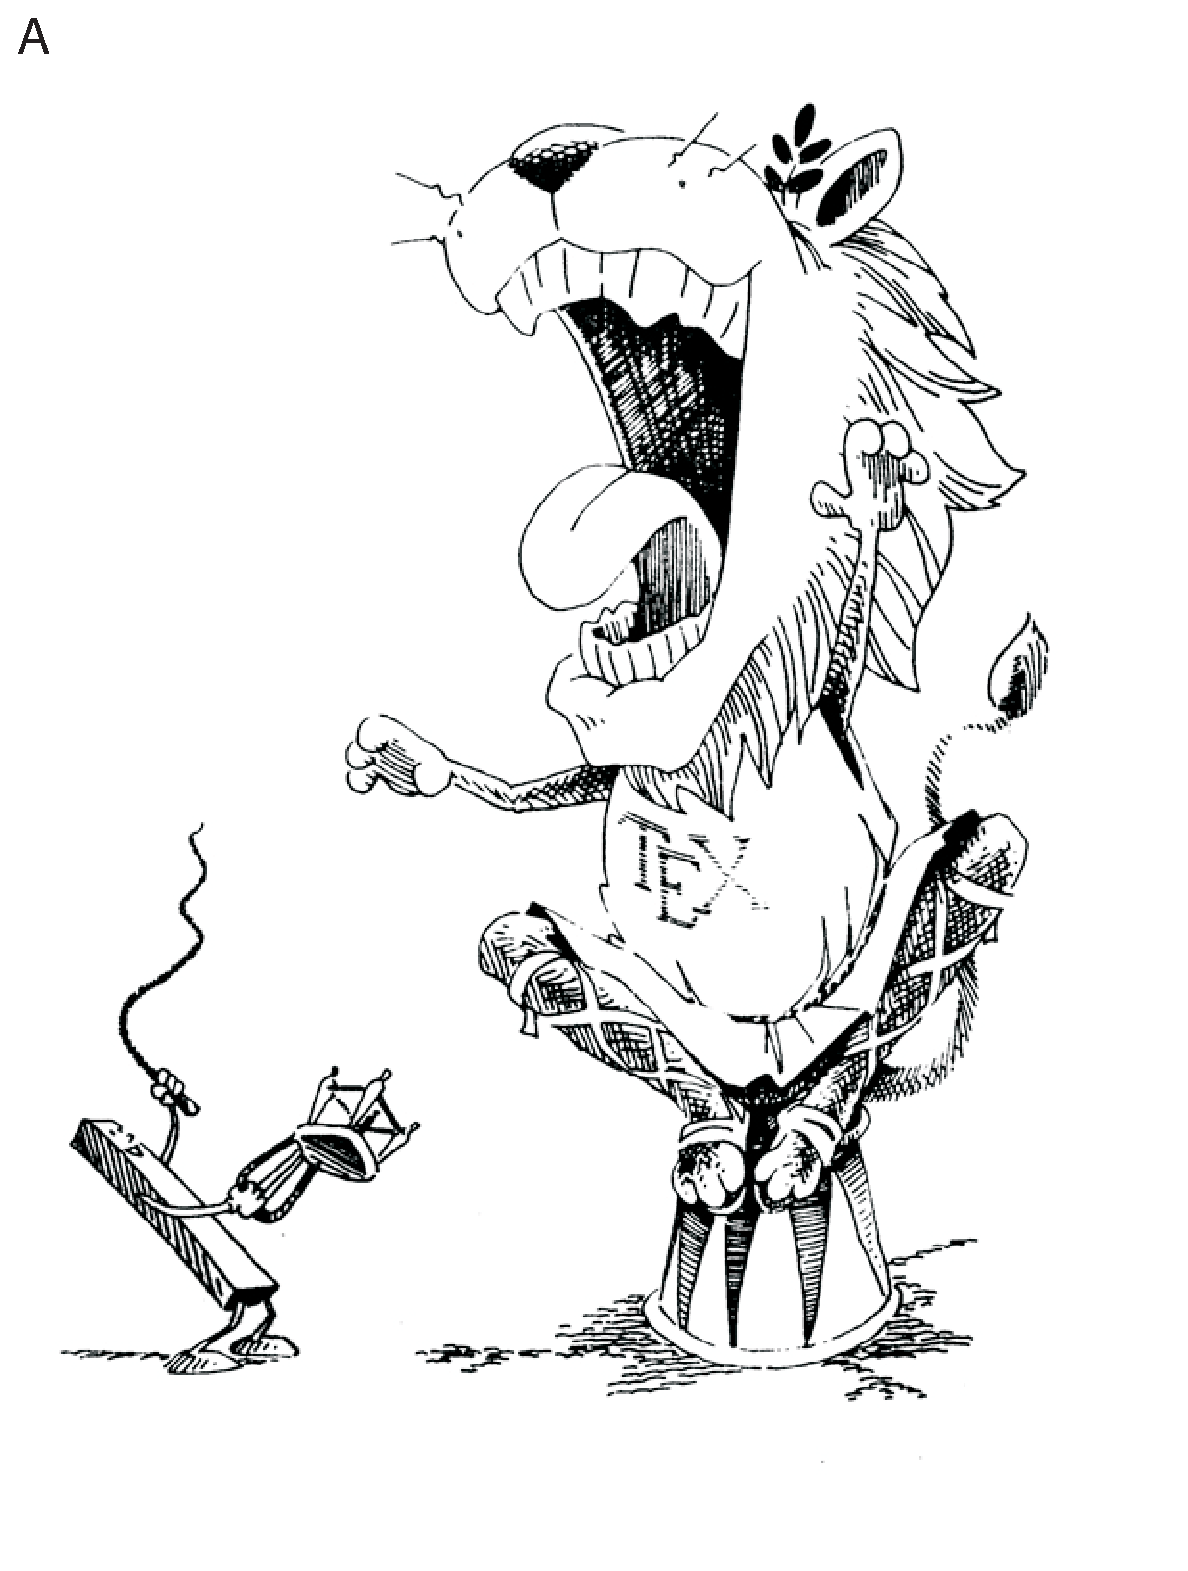
\includegraphics[width=0.5\columnwidth]{Controlling_TeX}}
		\caption{Você já aprendeu a controlar o \LaTeX?}
		\label{fig:knuth}
	\end{figure}	

%----------------------------------
% RESULTS AND DISCUSSION
%----------------------------------
\section{RESULTS AND DISCUSSION}\label{sec:results}

	According to the theoretical model for a highly mobile two-dimensional electron gas in double-quantum-wells, the magnetic field dependence of the localization correction in respect of the conductivity under diffusive condition ($B < B_{tr}$) is described by the following expression:
	\begin{equation}\label{eq:sigmaxB}
		\Delta\sigma(B) = \frac{e^2}{4\pi^2\hbar} \left[
		F\left(\frac{B/B_{tr}}{\tau/\tauphi}\right) +
		F\left(\frac{B/B_{tr}}{\tau/\tauphi + 2\tau/\ttau}\right) \right]\text{,}
	\end{equation}
	where the function $F(x) = \Psi(1/2 + 1/x) + \ln(x)$, $\Psi$ is the di-gamma function and $B_{tr} = \hbar/\left(4eD\tau\right)$ is the transport field.	$D$ is the diffusion coefficient. The variation of magnetoconductivity at	different temperatures for zero gate bias is shown in Fig.~\ref{fig:knuth} and that at $T = \unit{0.5}{\kelvin}$ for different gate biases is shown in Fig.~\ref{fig:knuth}. The symbols represent the experimental data and the solid curves are the theoretical predictions obtained from eq.~\eqref{eq:sigmaxB}. So, the WL predictions describe our experimental data well. The average dephasing scattering time $\tauphi$ and tunneling time $\ttau$ have been determined from the fits on the plots of MC and the formulae predicted by the WL theories. As expected, we observed that the dephasing scattering time depends strongly on temperature, but the tunneling time is independent of temperature.
		
%----------------------------------
% ACKNOWLEDGMENTS
%----------------------------------
\section{ACKNOWLEDGMENTS}
	Support of this work by FAPESP and CNPq (Brazilian agencies) is thankfully acknowledged. AKM thanks the FAPESP for providing all kind of financial supports, including his travel and sustenance allowances.

%----------------------------------
% BIBLIOGRAPHY
%----------------------------------
\begin{thebibliography}{++}
	\bibitem{Abrahams:1979} E. Abrahams, P. W. Anderson, D. C. Licciardellow and T. V. Ramakrishnan, Phys. Rev. Lett. \textbf{42}, 673 (1979).
	
	\bibitem{Anderson:1980} P. W. Anderson, D. J. Thouless, E. Abrahams and D. S. Figher, Phys. Rev. B \textbf{22}, 3519 (1980).
	
	\bibitem{Hikami:1980} S. Hikami, A. I. Larkin and Y. Nagaoka, Prog. Theor. Phys. \textbf{63}, 707 (1980).	
\end{thebibliography}

\end{document}